% Part 2 - Literature study

\chapter{Video Game Theory}
\label{chapter:lit-study-game-theory}
\lhead{Chapter \ref{chapter:lit-study-game-theory}. \emph{Game Theory}}

This chapter looks at some previous articles on subjects related to video game theory with the goal of establishing a terminology to be used throughout the project.

\section{Game Types}

\todo{Item hunt games etc}

\section{Reward Systems}
\label{sec:reward-systems}

\todo{Rewards for progress, daily rewards etc}

\section{Player Types}

Player types are a way of categorizing players on various axes with the goal of creating an enjoyable game experience for the target audience. Identifying player types can also be important for developers of games whose business model is to sell in-game items rather than retail sale of the game itself, as Hamari \& Tuunanen \cite{hamari2014playertypes} discussed in their 2014 meta-synthesis on the subject. The design of such items is largely based on the potential customers, and what type of items will be sold will depend on who are going to play the game and what their motivations are.

There are countless studies on different player types, and Hamari \& Tuunanen \cite{hamari2014playertypes} compared the different ways previous researchers have segmented players to create their typologies, using primarily behavioral and psychographic segmentation, but sometimes also geographic or demographic segmentation.

They found that a common division was that of \emph{hardcore} and \emph{casual} players, but found this to be a too simplistic solution. Hardcore players were sometimes described to be more dedicated in all areas of the games, playing for longer sessions, more often and being more invested. However, they found that all these aspects and more were better treated separately, creating multiple scales used to define more than just two types of players.

Kallio et al. \cite{kallio2010gamermentalities} used a model consisting of the scales of \emph{Intensity} and \emph{Sociability}, along with a \emph{Games} component to define three different groups of gamer mentalities. The components of the model can be seen in Figure \ref{fig:kallio-gamer-mentalities-model}, as presented in their paper, and the three groups of mentalities they define using this model are \emph{Social mentality profiles}, \emph{Casual mentality profiles} and \emph{Commited mentality profiles}.

\begin{figure}[h]
	\centering
	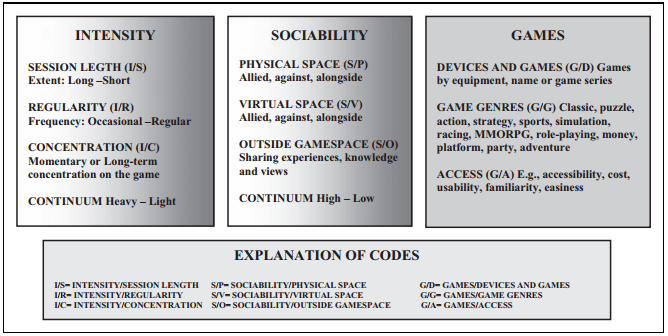
\includegraphics[width=\textwidth]{Figures/kallio-gaming-mentalities-model}
	\caption{The three components of gaming mentalities, as seen in Kallio et al. \cite{kallio2010gamermentalities}}
	\label{fig:kallio-gamer-mentalities-model}
\end{figure}

The social mentality profiles identified by Kallio et al. are of \emph{"quite light"} intensity, very high sociability and their choice in games focus on access to the games. The casual mentality profiles have variable intensity, low sociability and their choice in games focuses primarily on the device and access. The committed mentality profiles have \emph{"heavy"} intensity, high sociability and their choice in games focuses primarily on the genre. Each of the groups of profiles consist of three profiles with different, although similar, values for the various metrics defined in the model. \advice{Is this paragraph (or even source) really of any use here?}

Hamari \& Tuunanen \cite{hamari2014playertypes} used this and other papers to identify a total of five \emph{"key dimensions pertaining to motivations of play/orientation of the player"}: \emph{Achievement}, \emph{Exploration}, \emph{Sociability}, \emph{Domination} and \emph{Immersion}.

In this project, we will use the five archetypal player types \emph{Achieving}, \emph{Exploring}, \emph{Socializing}, \emph{Dominating} and \emph{Immersing}, where each of them is \emph{more concerned with} their respective dimension of the game than the four others, rather than \emph{entirely focused on} only that aspect. That is, for a \emph{Socializing} player, the social aspect of the game is more important than any other aspect, but they may still have varying interest in the other four dimensions.

\chapter{Game Types}
\label{chapter:lit-study-game-types}
\lhead{Chapter \ref{chapter:lit-study-game-types}. \emph{Game Types}}

\section{Location-Based, Augmented Reality, and Pervasive Games}
\label{sec:prestudy-ar-location-pervasive-games}

\section{Exergames}

\todo{Zombies Run, Stolpejakten, Munzee, Run an Empire}

\section{Mobile Games}
\label{sec:mobile-games}

\todo{Talk about typical mobile games, microtransactions etc}

\section{Similar Games}

\todo{Ingress, Geocaching, ++}


% Chapter - More about Pokémon and Pokémon GO
\chapter{Pokémon GO}
\label{chapter:lit-study-pokemon-go}
\lhead{Chapter \ref{chapter:lit-study-pokemon-go}. \emph{Pokémon GO}}

\section{Pokémon Franchise}
\todo{Short introduction to the Pokémon franchise, some terms and the different games?}

\section{Pokémon GO In-Depth}
\label{sec:pokemon-go-in-depth}
\todo{Tech choices for GO and differences from "main" games}

\section{Pokémon GO and Video Game Theory}
\label{sec:pokemon-go-theory}
\todo{Elaborate on Pokémon GO with the theory from this chapter.}


% Chapter - Current state of physical and mental health in society (western world?)
\chapter{Modern Society and Health}
\label{chapter:lit-study-modern-health}
\lhead{Chapter \ref{chapter:lit-study-modern-health}. \emph{Modern Society and Health}}

\section{Physical Activity}
\label{sec:lit-study-physical-activity}

\todo{About increasingly sedentery lifestyles in modern society, the effects of just moving a little every day etc}

\section{Mental Health}
\label{sec:lit-study-mental-health}

\todo{About the effects of gaming (having fun, accomplishing goals), being social, and exercising}

